\documentclass[10pt,twocolumn,letterpaper]{article}

\usepackage{cvpr}
\usepackage{microtype}
\usepackage{multirow}
\usepackage{array}
\usepackage{tikz}
\usepackage{placeins}
\usepackage{float}
\usetikzlibrary{arrows.meta,positioning,fit,backgrounds}
\usepackage[hidelinks]{hyperref}

% ---------- Compact but safe float spacing ----------
\setlength{\textfloatsep}{5pt plus 1pt minus 1pt}
\setlength{\floatsep}{5pt plus 1pt minus 1pt}
\setlength{\intextsep}{5pt plus 1pt minus 1pt}
\setlength{\dbltextfloatsep}{5pt plus 1pt minus 1pt}
\setlength{\dblfloatsep}{5pt plus 1pt minus 1pt}
\setlength{\abovecaptionskip}{3pt}
\setlength{\belowcaptionskip}{1pt}
\setlength{\columnsep}{0.24in}

\makeatletter
\setlength{\@fptop}{0pt}
\setlength{\@fpsep}{5pt plus 1pt minus 1pt}
\setlength{\@fpbot}{0pt plus 1fil}
\makeatother

\makeatletter
\def\cvprsection{\@startsection {section}{1}{\z@}
   {-10pt}{7pt} {\large\bfseries}}
\def\cvprssect#1{\cvprsection*{#1}}
\def\cvprsect#1{\cvprsection{\texorpdfstring{\hskip -1em.~}{}#1}}
\def\section{\@ifstar\cvprssect\cvprsect}

\def\cvprsubsection{\@startsection {subsection}{2}{\z@}
   {-8pt}{5pt} {\normalsize\bfseries}}
\def\cvprssubsect#1{\cvprsubsection*{#1}}
\def\cvprsubsect#1{\cvprsubsection{\texorpdfstring{\hskip -1em.~}{}#1}}
\def\subsection{\@ifstar\cvprssubsect\cvprsubsect}

\def\cvprsubsubsection{\@startsection {subsubsection}{3}{\z@}
   {-6pt}{3pt} {\normalsize\bfseries}}
\def\cvprssubsubsect#1{\cvprsubsubsection*{#1}}
\def\cvprsubsubsect#1{\cvprsubsubsection{\texorpdfstring{\hskip -1em.~}{}#1}}
\def\subsubsection{\@ifstar\cvprssubsubsect\cvprsubsubsect}
\makeatother

\def\confName{COMP6242}
\def\confYear{2026}
\def\paperID{Final}

\title{From ImageNet to EuroSAT:\\Transfer Learning, Forgetting, and When Transfer Helps}
\author{
Ruiquan Qiao\\
{\small u8304432}
\and
Tiancheng Xia\\
{\small u8300865}
\and
Guangde Shi\\
{\small u8198083}
}
\date{}

\begin{document}
\raggedbottom
\twocolumn[{
\maketitle

\vspace{-1.2em}
\noindent\hfill
\begin{minipage}{0.88\textwidth}
\hrule
\vspace{0.65em}
\footnotesize
\centering\textbf{Author Contributions and AI Usage Statement}\par
\vspace{0.35em}
\raggedright
\textbf{Ruiquan Qiao:} main EuroSAT experiment, main forgetting analysis, report integration, code baseline design, ImageNet data processing for the catastrophic forgetting experiments, and style alignment between the presentation slides and the paper.\\
\textbf{Tiancheng Xia:} same-size cross-domain experiment, domain-gap forgetting analysis, discussion of when transfer helps except the data-size study, code unification and refactoring, integration of course concepts into the report, and detailed report revision.\\
\textbf{Guangde Shi:} EuroSAT data-size experiment, data-size forgetting analysis, related result discussion, detailed discussion of when transfer helps in the data-size setting, improvement of experimental result visualizations, and video preparation.\\
\textbf{AI Usage Statement:} AI tools supported language refinement, LaTeX formatting, figure preparation, and report drafting; the experimental design, code execution, result interpretation, and final decisions were verified by the group.\\
\textbf{Source Code:} \url{https://github.com/RuiquanQiao/COMP6242-group-project}
\vspace{0.65em}
\hrule
\end{minipage}
\hfill\mbox{}
\vspace{1.35em}
}]

\begin{abstract}
This project studies when ImageNet pretraining helps downstream visual recognition and what it costs after adaptation. Using ResNet-18, the experiments compare training from scratch, linear probing, partial unfreezing, and full fine-tuning on EuroSAT, then extend the analysis with a CIFAR-10 domain-gap comparison, a EuroSAT data-size study, and ImageNet re-evaluation for catastrophic forgetting. The results show that transfer learning improves EuroSAT classification when the pretrained backbone is allowed to adapt, with partial unfreezing providing the strongest accuracy-efficiency trade-off among the evaluated strategies. Transfer is most useful when labelled target data are limited or when the target domain is closer to ImageNet, but stronger adaptation also causes severe forgetting on the original ImageNet task. These findings highlight a practical trade-off between downstream accuracy and source-task retention.
\end{abstract}

\section{Introduction}
ImageNet pretraining is often treated as a reliable starting point for vision tasks, but this assumption becomes less obvious when the target images are satellite scenes rather than object-centric photographs. EuroSAT images are viewed from above and are defined by land-cover patterns, texture, and spatial layout, so the features learned from ImageNet may not transfer automatically \cite{russakovsky2015,deng2009,cheng2020,helber2019}.

This project studies that problem by adapting an ImageNet-pretrained ResNet-18 \cite{he2016,deng2009} to EuroSAT \cite{helber2019} and comparing it with training from scratch. We test linear probing, partial unfreezing, and full fine-tuning to understand how much of the pretrained model should be frozen or updated.

Beyond the main EuroSAT experiment, we ask when transfer helps and what it costs. We compare EuroSAT with CIFAR-10 under the same sample budget \cite{krizhevsky2009}, vary the amount of EuroSAT training data, and evaluate ImageNet performance after downstream adaptation to measure catastrophic forgetting on the original source task \cite{goodfellow2013,russakovsky2015}.

\section{Related Work}
ImageNet-pretrained models are widely used as starting points for transfer learning because large-scale supervised training produces reusable visual features \cite{russakovsky2015,deng2009}. However, transfer quality depends on task distance, and earlier layers tend to be more general than later layers \cite{yosinski2014}. This motivates our comparison of linear probing, partial unfreezing, and full fine-tuning.

Remote sensing scene classification is a useful stress test for transfer because its classes are defined by overhead land-cover patterns rather than object-centric appearance \cite{cheng2020}. EuroSAT provides a standard benchmark for this setting with 27,000 Sentinel-2 image patches across 10 classes \cite{helber2019}.

Fine-tuning also raises the issue of catastrophic forgetting: performance on a previous task can drop after training on a new task \cite{goodfellow2013}. Although methods such as EWC and Learning without Forgetting address this problem \cite{kirkpatrick2017,li2016}, our focus is to measure how much ordinary downstream fine-tuning changes the original ImageNet capability.

\section{Experimental Setup}
\newcommand{\workflowfigure}{%
\begin{figure}[!htbp]
\centering
\resizebox{\columnwidth}{!}{%
\begin{tikzpicture}[
  font=\small\sffamily,
  >=Latex,
  line width=0.9pt,
  box/.style 2 args={
    rounded corners=10pt,
    draw=##1!70!black,
    fill=##1!10,
    text width=##2,
    align=center,
    inner sep=6pt,
    minimum height=1.5cm,
  },
  arr/.style={->, draw=black!70, line width=1.0pt, shorten >=2pt, shorten <=2pt},
  dashedarr/.style={->, draw=black!55, dashed, line width=1.0pt, shorten >=2pt, shorten <=2pt},
  lane/.style={font=\scriptsize\sffamily\bfseries, text=black!55},
  group/.style={draw=black!45, dashed, rounded corners=10pt, inner sep=10pt}
]

\node[lane] at (0.0,1.2) {MAIN LINE};

\node[box={blue}{4.2cm}, minimum height=1.5cm] (source) at (0.0,0.0) {%
\textbf{ImageNet ResNet-18}\\
pretrained initialization};

\node[box={green!60!black}{4.2cm}, minimum height=1.5cm] (transfer) at (0.0,-2.3) {%
\textbf{Transfer to EuroSAT}};

\node[box={violet}{2.5cm}, minimum height=1.0cm] (scratch) at (-4.8,-5.6) {Scratch};
\node[box={violet}{2.5cm}, minimum height=1.0cm] (linearprobe) at (-1.6,-5.6) {Linear probe};
\node[box={violet}{2.5cm}, minimum height=1.0cm] (partialft) at (1.6,-5.6) {Partial unfreeze};
\node[box={violet}{2.5cm}, minimum height=1.0cm] (fullft) at (4.8,-5.6) {Full fine-tune};
\node[group, fit=(scratch) (linearprobe) (partialft) (fullft)] (strategygroup) {};
\node[font=\small\sffamily\bfseries, anchor=south west] at (strategygroup.north west) {4 Strategies};

\node[box={orange}{3.1cm}, minimum height=1.15cm] (mainexp) at (0.0,-9.6) {%
\textbf{4.1 Main Experiment}\\
EuroSAT ablation};

\node[box={orange}{3.1cm}, minimum height=1.15cm] (domain) at (-4.0,-9.6) {%
\textbf{4.2 When Transfer Helps}\\
same-size domain gap};

\node[box={orange}{3.1cm}, minimum height=1.15cm] (fraction) at (4.0,-9.6) {%
\textbf{4.3 When Transfer Helps}\\
same-domain data size};
\node[group, fit=(mainexp) (domain) (fraction)] (studygroup) {};
\node[font=\small\sffamily\bfseries, anchor=south west] at (studygroup.north west) {When Transfer Helps};

\node[box={red}{2.7cm}, minimum height=1.1cm] (forgetmain) at (0.0,-13.0) {%
\textbf{5.1 Forgetting}\\
after main experiment};

\node[box={red}{2.7cm}, minimum height=1.1cm] (forgetdomain) at (-4.0,-13.0) {%
\textbf{5.2 Forgetting}\\
after domain gap};

\node[box={red}{2.7cm}, minimum height=1.1cm] (forgetfraction) at (4.0,-13.0) {%
\textbf{5.3 Forgetting}\\
after data size};
\node[group, fit=(forgetmain) (forgetdomain) (forgetfraction)] (forgetgroup) {};
\node[font=\small\sffamily\bfseries, anchor=south west] at (forgetgroup.north west) {Catastrophic Forgetting};
\coordinate (strategytop) at (0,-4.66);
\coordinate (strategybottom) at (0,-6.54);
\coordinate (studytop) at (0,-8.32);
\coordinate (studybottom) at (0,-10.88);
\coordinate (forgettop) at (0,-12.00);
\draw[arr] (source.south) -- (transfer.north);
\draw[arr] (transfer.south) -- (strategytop);
\draw[arr] (strategybottom) -- (studytop);
\draw[dashedarr] (studybottom) -- (forgettop);
\end{tikzpicture}%
}
\caption{Experimental workflow used in Sections~4 and~5. The downstream experiments compare transfer strategies, target-domain distance, and training-set size. The downstream-trained checkpoints are then re-evaluated on ImageNet to measure catastrophic forgetting.}
\label{fig:pipeline}
\vspace{0.15em}
\end{figure}
}

\subsection{Backbone and Initialization}
All experiments use ResNet-18 \cite{he2016}. Transfer runs start from the official torchvision ImageNet-1K weights, while training from scratch uses random initialization. ResNet-18 first extracts local visual patterns through convolutional layers, then builds increasingly task-specific representations through deeper residual blocks. In this structure, earlier layers tend to capture general low-level features such as edges, corners, and textures, while later layers combine them into higher-level semantic patterns. The final fully connected layer maps the learned representation to class logits, so it must be replaced when the number of target classes changes.

For EuroSAT and CIFAR-10, the original 1000-way ImageNet classifier is replaced with a 10-way classifier. For ImageNet forgetting evaluation, the model is rebuilt with the original 1000-way head and the downstream-adapted backbone is loaded back into it. This allows us to test whether the feature extractor remains compatible with the original ImageNet task after downstream training.

We compare four strategies that update different parts of the network. Training from scratch updates the entire randomly initialized model and serves as the no-transfer baseline. Linear probing freezes the pretrained backbone and trains only the new classifier, testing whether ImageNet features are already separable for the target task. Partial unfreezing keeps most of the pretrained backbone frozen, but unfreezes the final residual stage of ResNet-18 and the new classifier; this allows higher-level features to adapt while keeping earlier visual filters fixed. Full fine-tuning updates the entire pretrained network, giving the model maximum flexibility but also the greatest risk of overwriting source-task representations. For the 10-class downstream tasks, ResNet-18 has 11,181,642 parameters after the classifier is replaced. Linear probing trains only the 10-class classifier, with $512 \times 10 + 10 = 5,130$ weights and biases. Partial unfreezing trains that classifier plus the final residual stage, giving 8,398,858 trainable parameters, while training from scratch and full fine-tuning both update all 11,181,642 parameters.

\workflowfigure

\subsection{Data Preparation}
The main downstream dataset is EuroSAT \cite{helber2019}, using a fixed class-balanced split of 27,000 RGB images into 18,900 train, 4,050 validation, and 4,050 test samples. The same split sizes are used for the CIFAR-10 same-size comparison \cite{krizhevsky2009}, so the domain-gap experiment compares target domains under the same amount of supervision. For the data-size analysis, the EuroSAT validation and test splits stay fixed while the training set is reduced to 10\%, 30\%, 60\%, and 100\% of the full training pool. This design changes only the amount of training evidence, while keeping evaluation conditions unchanged. For forgetting, the previous task is the original ImageNet-1K problem, evaluated on the official ILSVRC2012 validation set prepared in ImageFolder format.

All inputs are resized to $224 \times 224$ because ResNet-18 pretrained on ImageNet expects image tensors at this scale. EuroSAT and CIFAR-10 training use random horizontal flip and random rotation as data augmentation. These transformations expose the model to small appearance variations and reduce overfitting, especially when the training set is limited. Validation and test data use deterministic preprocessing so that evaluation measures the learned model rather than random augmentation effects.

All datasets are converted to tensors and normalized with ImageNet mean and standard deviation. This is important for transfer learning because the pretrained ResNet-18 weights were learned under ImageNet-style input normalization; using the same scale keeps the input distribution compatible with the pretrained filters. ImageNet forgetting evaluation follows the standard resize-center-crop pipeline. Whenever a subset of a split is requested, sampling is class balanced so that accuracy and Macro-F1 are not dominated by class-frequency differences.

\subsection{Training Protocol and Metrics}
To make the strategy comparisons controlled, we keep the main optimization protocol fixed across runs: seed 42, batch size 32, 8 training epochs, AdamW optimization, learning rate $3 \times 10^{-4}$, and weight decay $10^{-4}$. This means that the experimental variable is not the amount of training budget or a separate tuning recipe for each method, but the initialization and the subset of network parameters allowed to learn. Each training run follows the standard supervised learning pipeline: images are passed through the network to produce class logits, cross-entropy loss compares these logits with the ground-truth labels, backpropagation computes gradients for the trainable parameters, and AdamW updates those parameters while applying weight decay regularization.

Validation is used to monitor generalization during training. The best checkpoint is selected by validation top-1 accuracy rather than final-epoch accuracy, because the validation set gives an estimate of performance on unseen data and reduces dependence on a single last epoch.

Top-1 accuracy is the primary metric throughout the report because all downstream tasks are single-label classification tasks with balanced sampling. Top-1 accuracy is defined as the percentage of samples whose highest-probability prediction matches the ground-truth label. Macro-F1 is reported as a secondary check of class-balanced performance in the main strategy, domain-gap, and corresponding forgetting experiments. The data-size experiments focus on top-1 trends for compactness. To quantify the benefit of transfer learning, we define transfer gain as:
\( \text{Gain}=A_{\text{transfer}}-A_{\text{scratch}},\)
where $A_{\text{transfer}}$ is the downstream test accuracy obtained by a transfer-learning strategy and $A_{\text{scratch}}$ is the corresponding accuracy achieved when training from random initialization. To quantify catastrophic forgetting, we define forgetting as:
\( \text{Forgetting}=A_{\text{before}}-A_{\text{after}},\)
where $A_{\text{before}}$ is the original ImageNet top-1 accuracy of the pretrained model and $A_{\text{after}}$ is the ImageNet top-1 accuracy measured after downstream adaptation. Larger forgetting values indicate greater loss of source-task performance under the original ImageNet evaluation protocol.

\subsection{Experiment Structure}
The study has one main experiment and two supporting analyses. Section~4.1 compares four transfer strategies on EuroSAT. Section~4.2 studies when transfer helps by comparing EuroSAT and CIFAR-10 at the same sample size. Section~4.3 studies when transfer helps by varying the amount of EuroSAT training data. Chapter~5 then evaluates the resulting checkpoints on the official ImageNet validation set to measure catastrophic forgetting.

\section{Experiments and Results}
\subsection{Main Experiment: EuroSAT Strategy Ablation}
Section~4.1 asks the core question of the project: on EuroSAT, does ImageNet pretraining help ResNet-18, and which transfer strategy works best? We compare training from scratch, linear probing, partial unfreezing, and full fine-tuning under the same training budget.

\begin{table}[!htbp]
\centering
\small
\caption{EuroSAT strategy ablation.}
\label{tab:main}
\resizebox{\columnwidth}{!}{%
\begin{tabular}{lrrrrr}
\toprule
Strategy & Top-1 & Macro-F1 & Gain & Time (s) & Params \\
\midrule
Scratch & 93.21 & 93.04 & -- & 1100.5 & 11,181,642 \\
Linear probe & 88.54 & 88.33 & -4.67 & 560.2 & 5,130 \\
Partial unfreeze & \textbf{97.78} & \textbf{97.71} & \textbf{+4.57} & 641.2 & 8,398,858 \\
Full fine-tune & 97.56 & 97.50 & +4.35 & 1068.3 & 11,181,642 \\
\bottomrule
\end{tabular}}
\end{table}

\begin{figure}[!htbp]
\centering
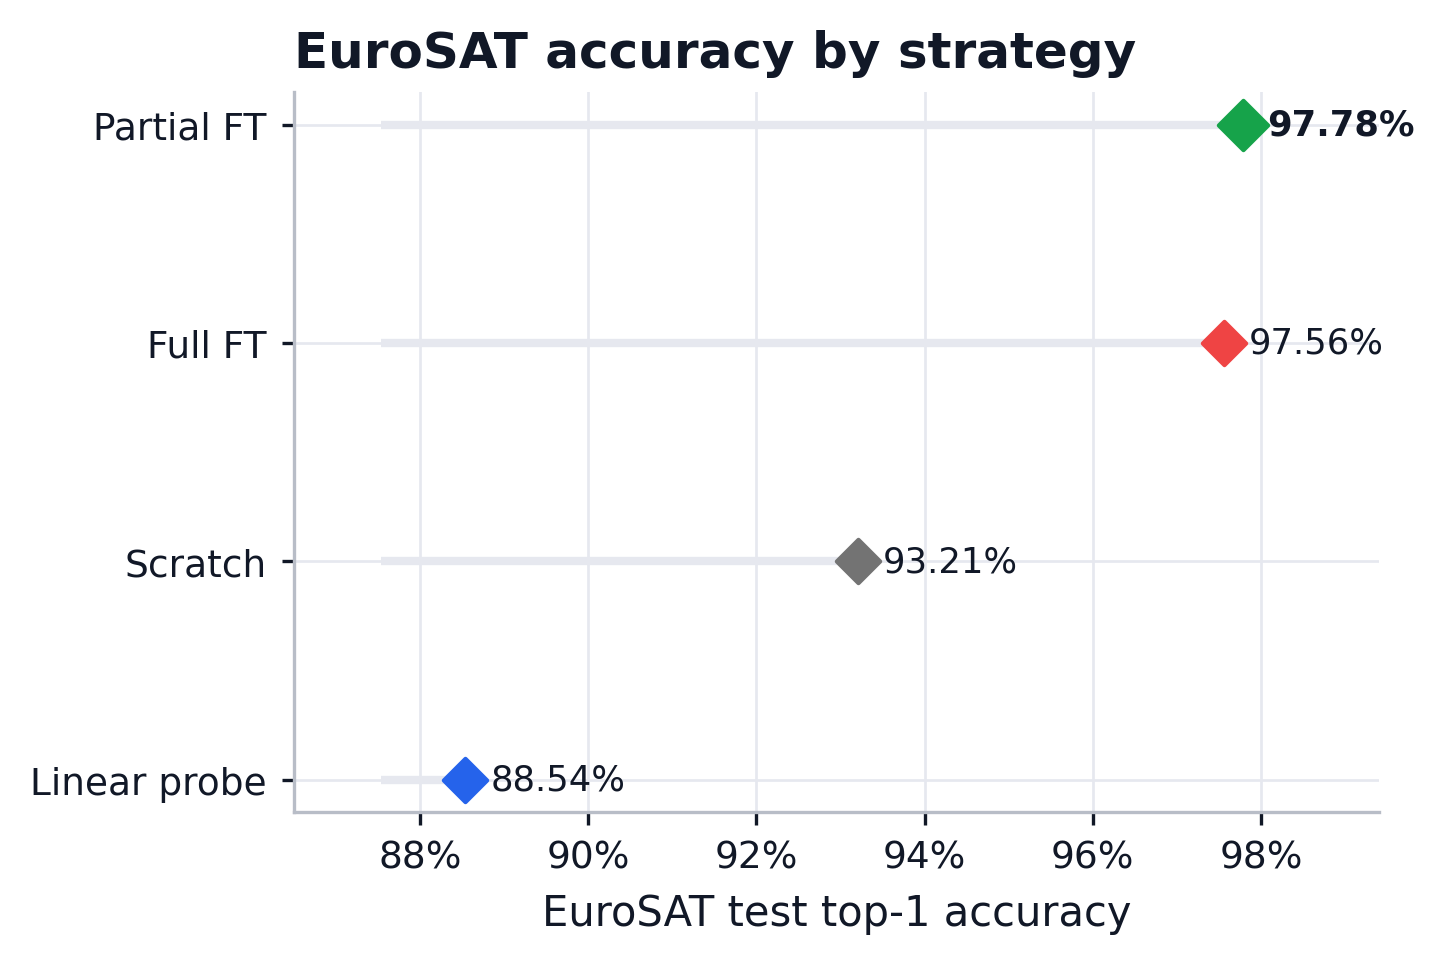
\includegraphics[width=0.84\columnwidth]{../outputs/new_style_picture/eurosat_ablation/test_top1_acc.png}
\vspace{0.1em}
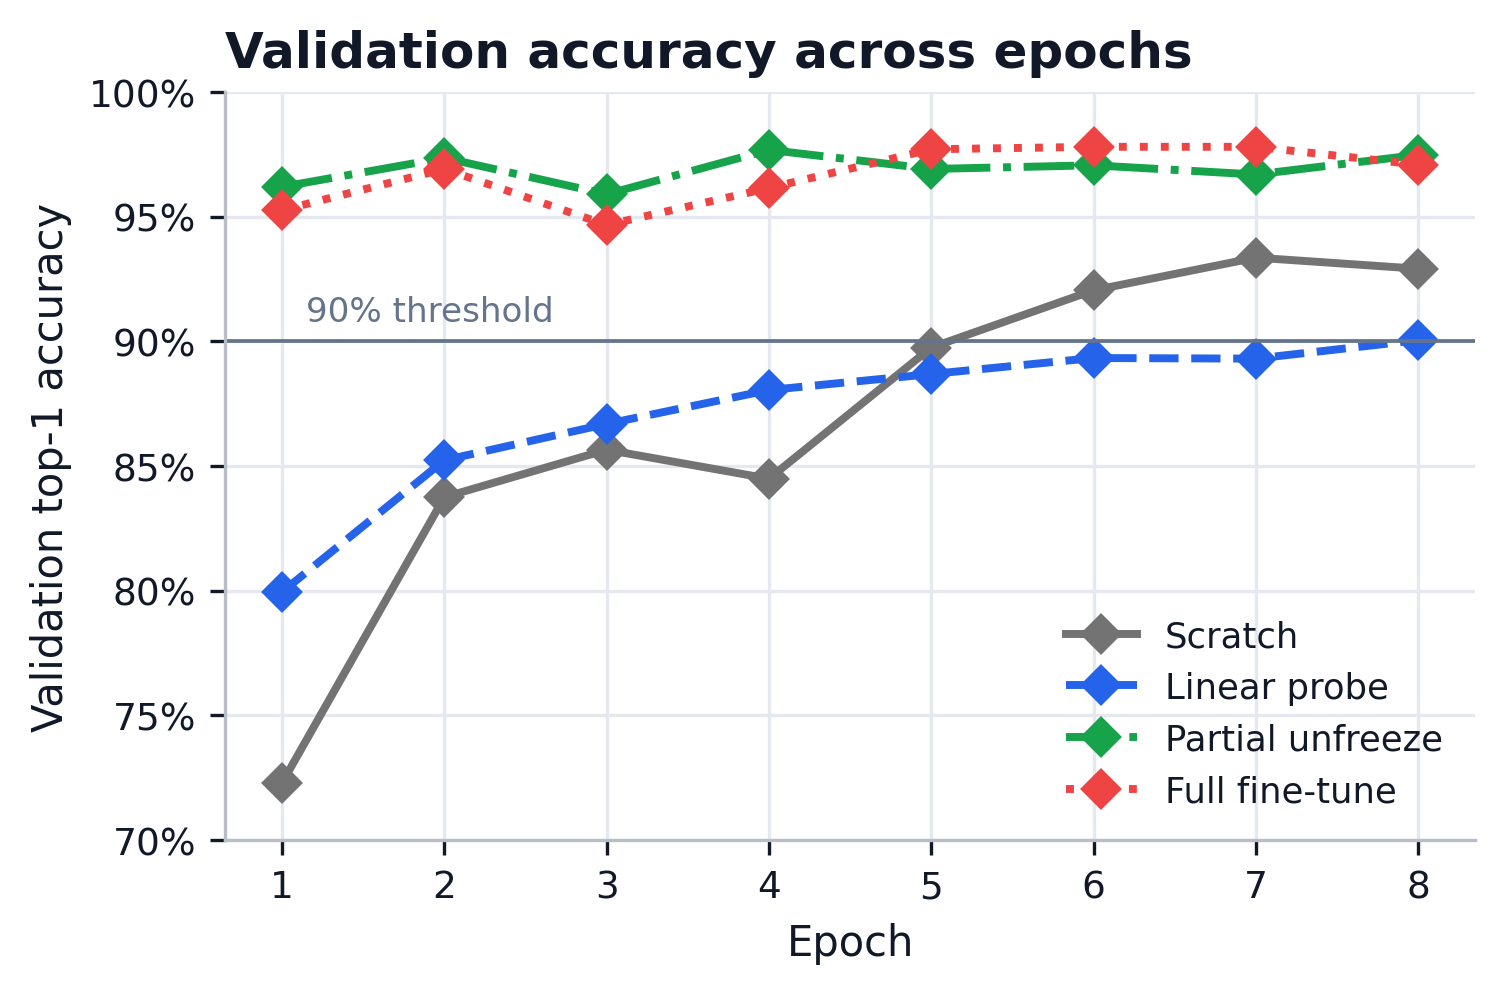
\includegraphics[width=0.84\columnwidth]{../outputs/new_style_picture/eurosat_ablation/val_top1_acc_curve.png}
\caption{Summary of Experiment 4.1. Top: final EuroSAT test top-1 accuracy by strategy. Bottom: validation top-1 trajectories across training epochs.}
\label{fig:main}
\end{figure}
The results show that transfer is helpful only when the pretrained model is allowed to adapt.
Partial unfreezing achieves performance comparable to full fine-tuning while requiring fewer trainable parameters and less computation, whereas linear probing is worst and even falls below the training-from-scratch baseline.


Partial unfreezing provides the strongest accuracy-efficiency trade-off in our experiments. It slightly outperforms full fine-tuning on the test set while using fewer trainable parameters and less training time, suggesting that adapting the top stage is sufficient for most of the domain shift. The convergence logs tell the same story: partial unfreezing and full fine-tuning pass the 90\% validation threshold in epoch 1, whereas training from scratch reaches it in epoch 6 and linear probing only in epoch 8.

Overall, the EuroSAT ablation shows that transfer is beneficial only when the backbone is allowed to adapt. Linear probing is insufficient for this domain shift, while partial unfreezing gives the strongest accuracy-efficiency trade-off.

\subsection{When Transfer Helps: Same-Size Cross-Domain Comparison}
This section compares EuroSAT and CIFAR-10 under the same sample budget in order to isolate the role of source-target domain similarity. Both datasets use 18,900 training, 4,050 validation, and 4,050 test samples, so the main difference is the target domain rather than the amount of supervision. EuroSAT represents a remote-sensing scene classification task with a clear shift from ImageNet, while CIFAR-10 remains closer to natural-image object recognition.

\begin{table}[!htbp]
\centering
\small
\caption{Cross-domain comparison.}
\label{tab:domain}
\resizebox{\columnwidth}{!}{%
\begin{tabular}{llrrr}
\toprule
Dataset & Strategy & Top-1 & Macro-F1 & Gain \\
\midrule
EuroSAT & Scratch & 92.86 & 92.67 & -- \\
EuroSAT & Linear probe & 88.54 & 88.33 & -4.32 \\
EuroSAT & Partial unfreeze & \textbf{97.51} & \textbf{97.41} & \textbf{+4.64} \\
EuroSAT & Full fine-tune & 97.31 & 97.25 & +4.44 \\
CIFAR-10 & Scratch & 78.12 & 78.27 & -- \\
CIFAR-10 & Linear probe & 78.20 & 78.00 & +0.07 \\
CIFAR-10 & Partial unfreeze & \textbf{91.19} & \textbf{91.18} & \textbf{+13.06} \\
CIFAR-10 & Full fine-tune & 90.07 & 90.03 & +11.95 \\
\bottomrule
\end{tabular}}
\end{table}

\begin{figure}[!htbp]
\centering
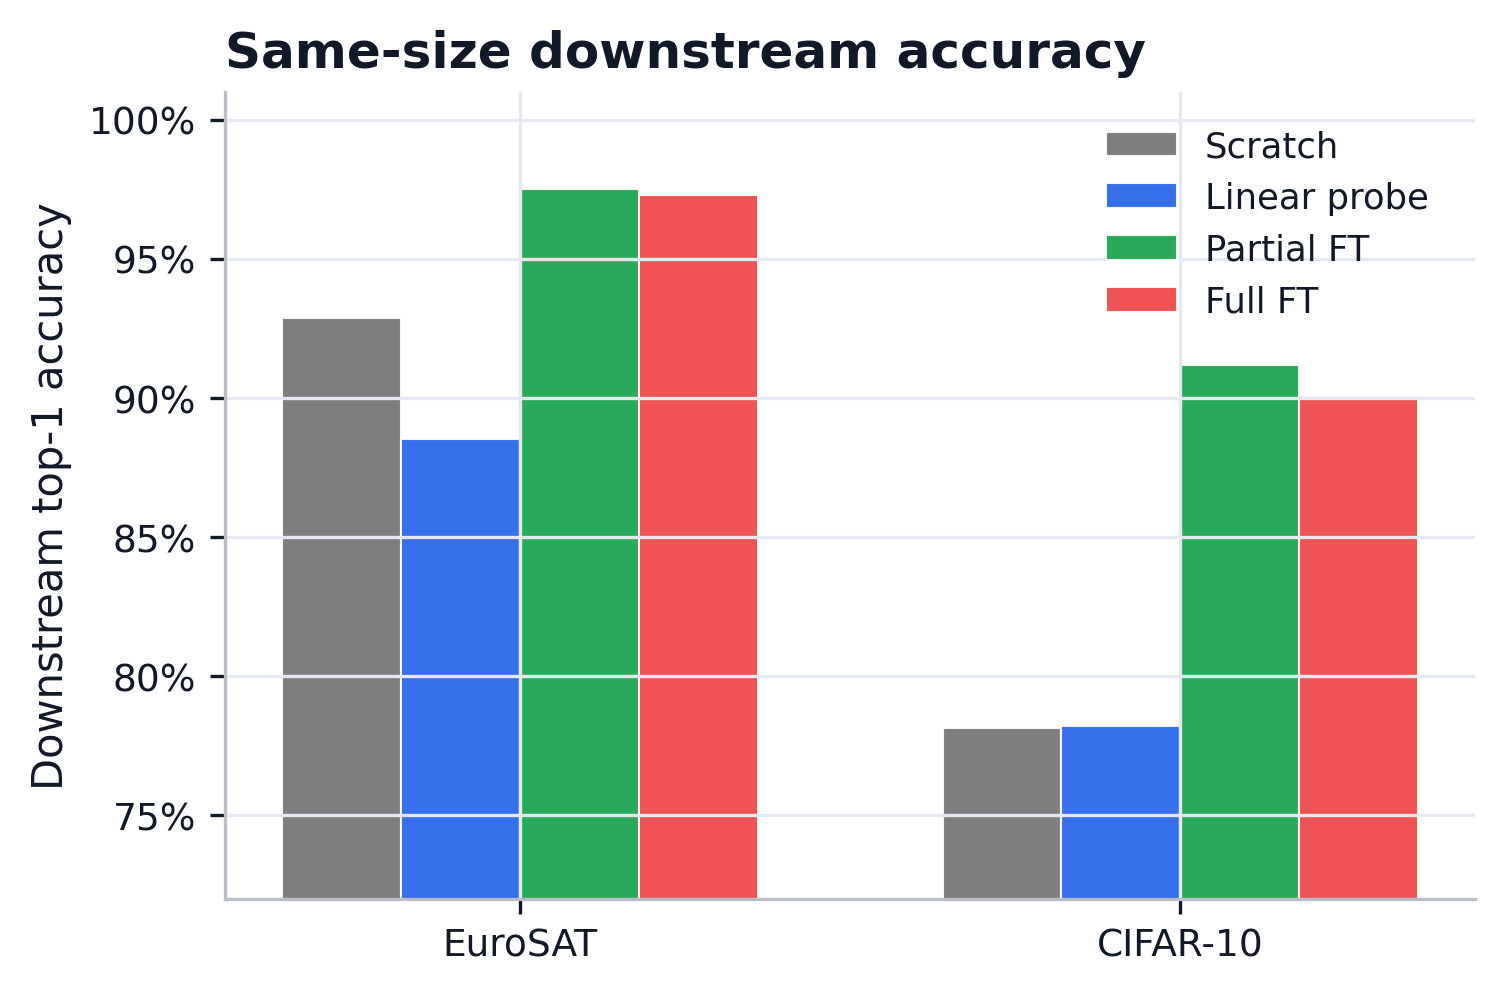
\includegraphics[width=0.78\columnwidth]{../outputs/new_style_picture/domain_gap/test_top1_acc.png}
\vspace{0.1em}
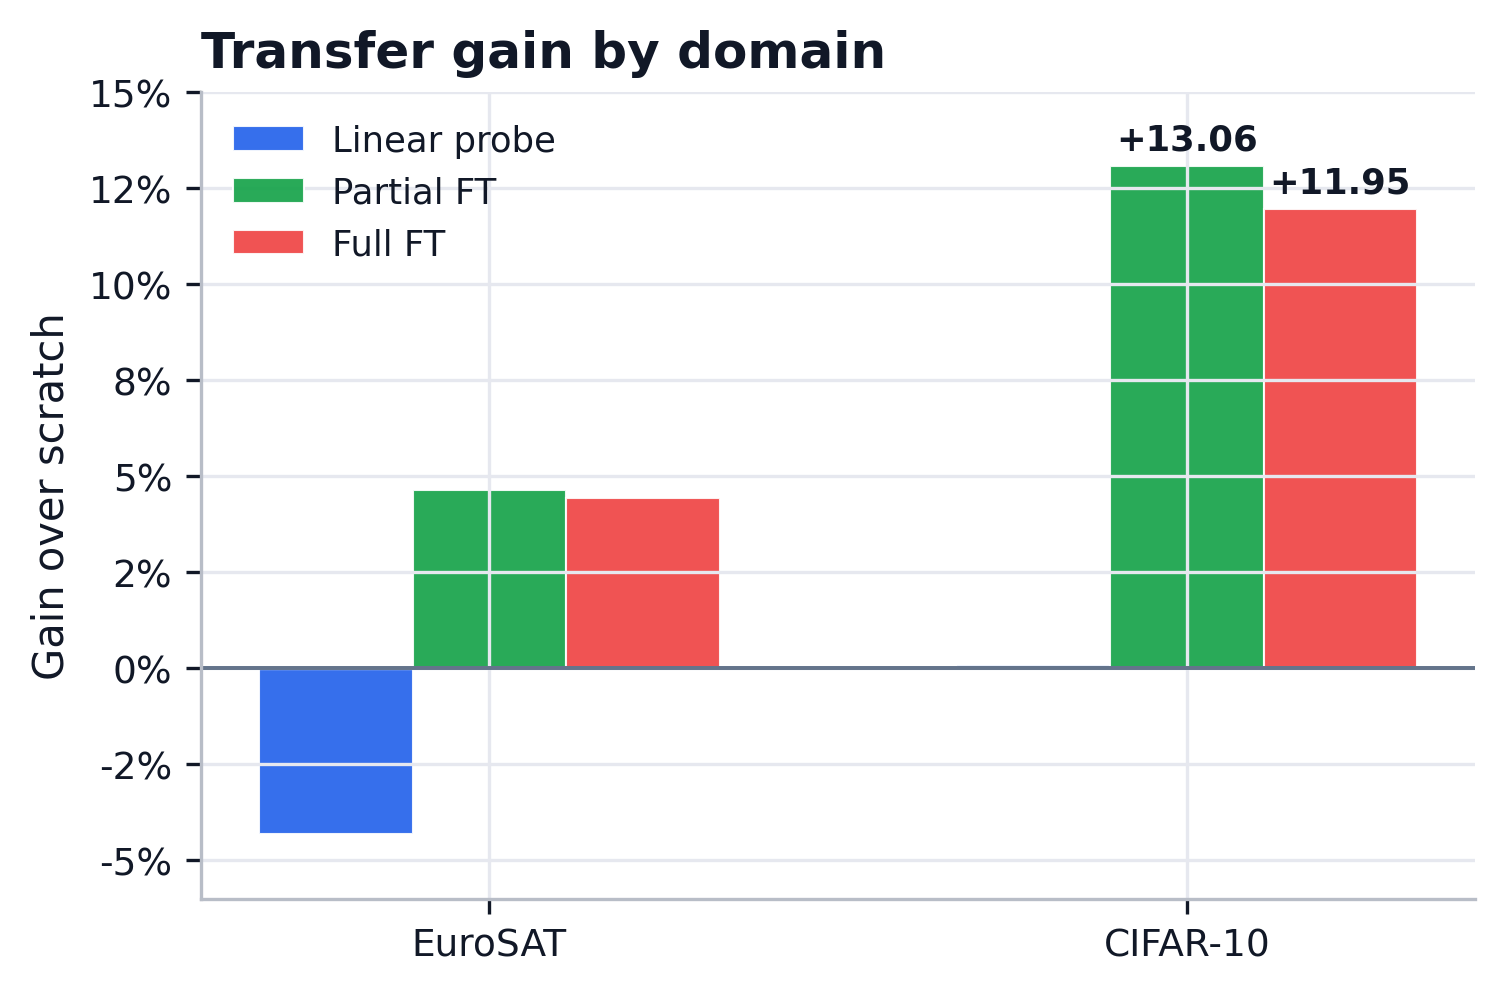
\includegraphics[width=0.78\columnwidth]{../outputs/new_style_picture/domain_gap/transfer_gain_top1.png}
\caption{Cross-domain comparison. Top: downstream test top-1 accuracy. Bottom: top-1 transfer gain over training from scratch.}
\label{fig:domain}
\end{figure}




The same-size comparison preserves the pattern observed in Section~4.1: transfer is most effective when the pretrained backbone is allowed to adapt. On EuroSAT, partial unfreezing and full fine-tuning improve accuracy by 4.64 and 4.44 percentage points over training from scratch, whereas the gains on CIFAR-10 are much larger (13.06 and 11.95 points).

Despite achieving lower absolute accuracy, CIFAR-10 benefits more from pretraining than EuroSAT. This result suggests that transferability depends not only on final task performance, but also on how effectively the task can be learned from scratch.


\subsection{When Transfer Helps: Same-Domain Data-Size Comparison}
This section varies the amount of EuroSAT training data in order to study whether transfer becomes more valuable in lower-data regimes. The model and target domain are fixed, while the EuroSAT training fraction is changed from 10\% to 30\%, 60\%, and 100\%. We compare training from scratch, linear probing, and full fine-tuning to represent no transfer, frozen-feature transfer, and full adaptation.

\begin{table}[!htbp]
\centering
\small
\caption{Same-domain EuroSAT data-size comparison.}
\label{tab:fraction}
\resizebox{\columnwidth}{!}{%
\begin{tabular}{rrrrr}
\toprule
Train \% & Scratch & Linear probe & Full fine-tune & Full fine-tune gain \\
\midrule
10 & 68.02 & 76.20 & \textbf{93.58} & +25.56 \\
30 & 82.83 & 85.10 & \textbf{96.65} & +13.82 \\
60 & 89.46 & 86.99 & \textbf{96.88} & +7.41 \\
100 & 89.39 & 87.93 & \textbf{97.15} & +7.75 \\
\bottomrule
\end{tabular}}
\end{table}


\begin{figure}[!htbp]
\centering
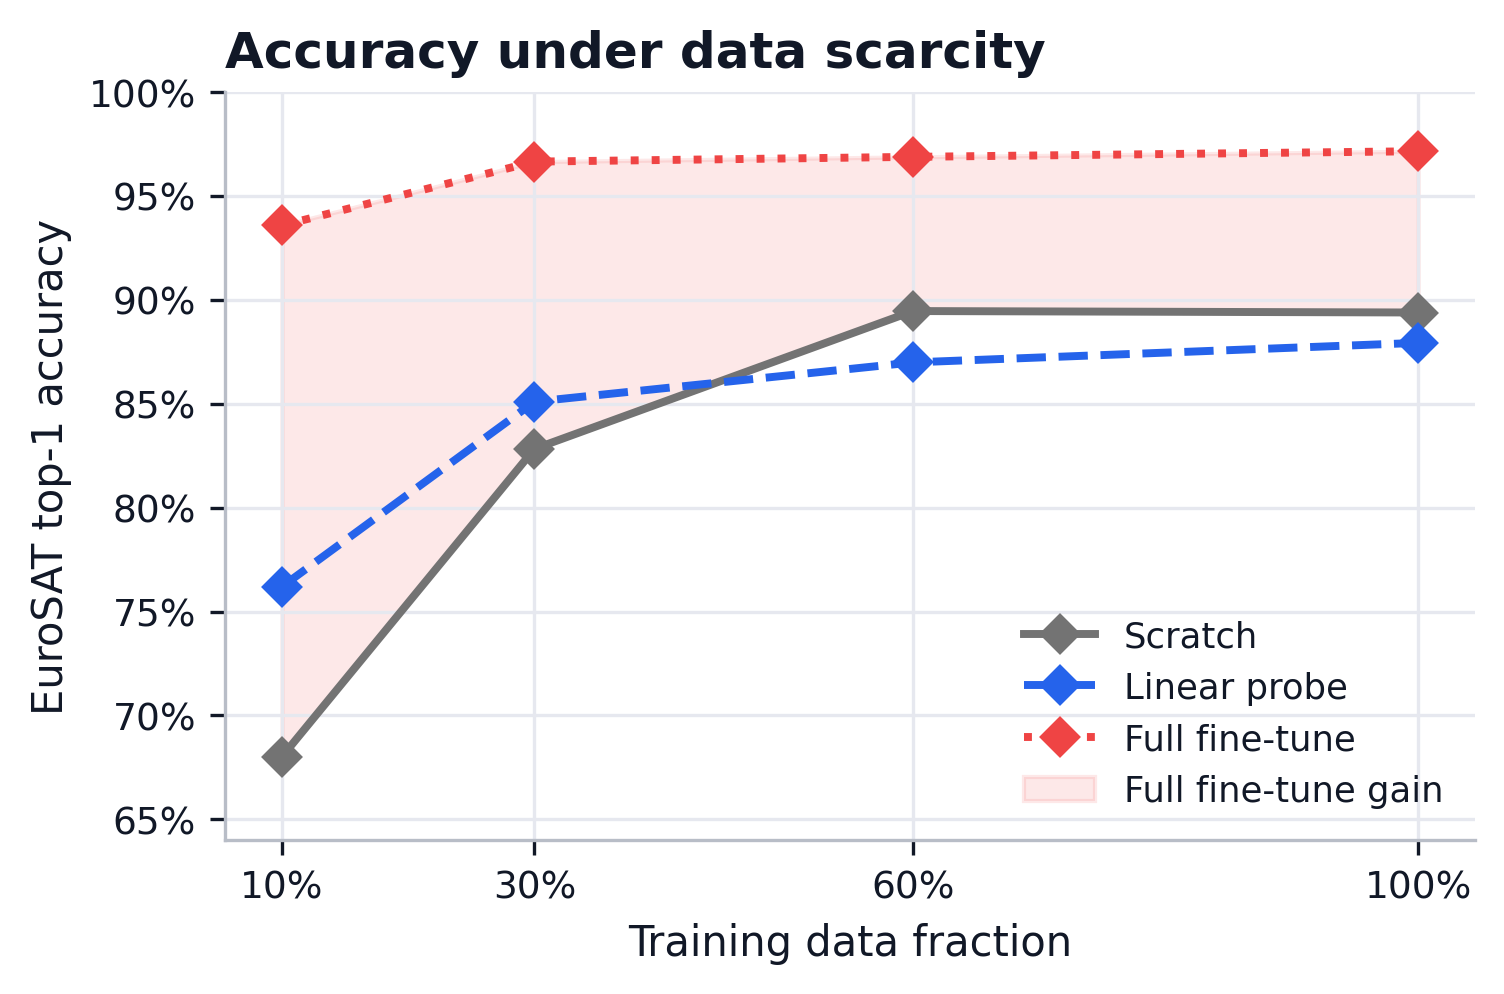
\includegraphics[width=0.78\columnwidth]{../outputs/new_style_picture/data_fraction/test_top1_acc.png}
\vspace{0.1em}
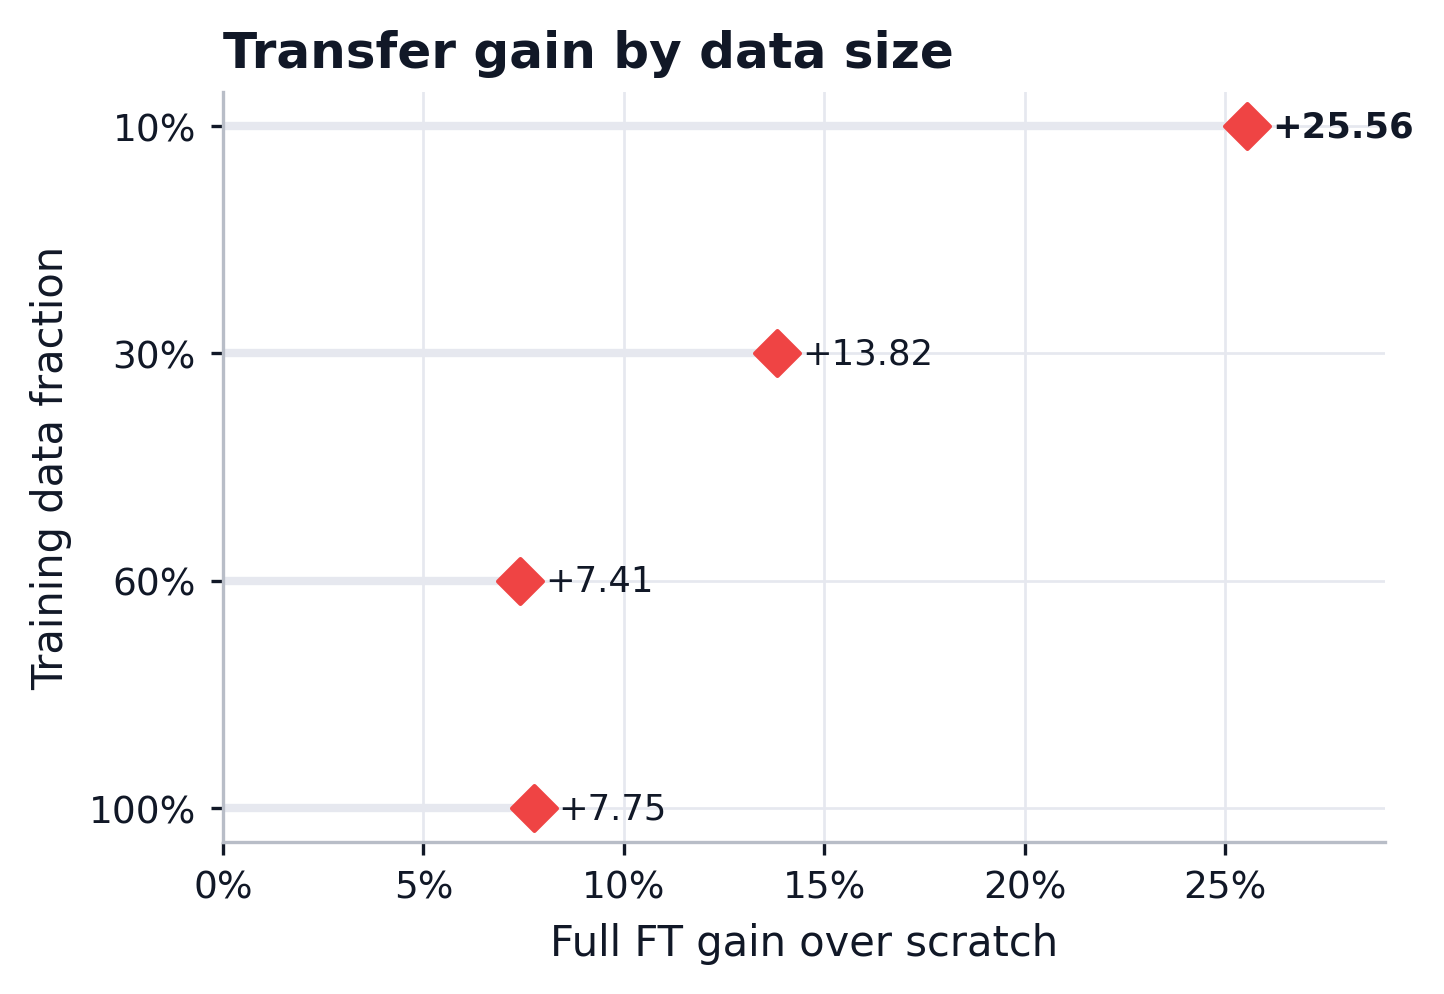
\includegraphics[width=0.78\columnwidth]{../outputs/new_style_picture/data_fraction/transfer_gain_top1.png}
\caption{Same-domain data-size comparison. Top: EuroSAT test top-1 accuracy by training fraction. Bottom: transfer gain over training from scratch.}
\label{fig:fraction}
\end{figure}

This experiment focuses on how performance changes with training-set size, we report top-1 accuracy and top-1 transfer gain as the primary trend metrics.

The results show that transfer is most valuable when labeled data is limited. With only 10\% of the EuroSAT training set, full fine-tuning improves over training from scratch by 25.56 percentage points. As the training fraction increases, the model trained from scratch becomes stronger, and the gain from full fine-tuning decreases to about 7--8 points. This shows that transfer mainly improves sample efficiency in this setting.

Linear probing helps at 10\% and 30\% data, but it becomes worse than training from scratch at 60\% and 100\%. The data-size trend shows that transfer is most valuable in the low-data regime; as more EuroSAT labels are available, training from scratch becomes stronger and the relative gain from full fine-tuning decreases.


\section{Catastrophic Forgetting Analysis}
Section~5 returns each downstream-adapted model to the official ILSVRC2012 validation set and measures how much of the original ImageNet capability has been lost after fine-tuning. Rather than introducing a new task, this section serves as a direct post-test for Section~4: Section~4 asks how well the model learns the downstream task, while Section~5 asks how much ImageNet performance is forgotten in the process.

In this section, a trade-off refers to the balance between downstream adaptation and source-task retention. A desirable model would achieve high downstream accuracy or transfer gain while keeping ImageNet forgetting low. In the scatter plot in Section~5.2, the horizontal axis is ImageNet forgetting and the vertical axis is downstream test accuracy, so points closer to the upper-left region are preferable. Points on the right side indicate stronger forgetting, even if their downstream accuracy is high. In Section~5.3, the trade-off is shown across training fractions by plotting transfer gain and forgetting as separate trends.

\subsection{Forgetting After the Main EuroSAT Experiment}
We evaluate the linear probing, partial unfreezing, and full fine-tuning checkpoints from Section~4.1 on the official ILSVRC2012 validation set. The original ImageNet-pretrained ResNet-18 obtains 69.76\% top-1 accuracy and 69.30 macro-F1 before downstream adaptation. For each strategy, forgetting is measured as the drop from this baseline to the EuroSAT-adapted model evaluated back on ImageNet. Training from scratch is excluded because it does not start from ImageNet-pretrained weights.

\begin{table}[!htbp]
\centering
\small
\caption{Forgetting after the main EuroSAT experiment.}
\label{tab:forget}
\resizebox{\columnwidth}{!}{%
\begin{tabular}{lrrrrr}
\toprule
Strategy & ImageNet After & Forgetting & After Macro-F1 & Forgetting F1 & EuroSAT Top-1 \\
\midrule
Linear probe & 32.03 & 37.73 & 33.87 & 35.43 & 88.54 \\
Partial unfreeze & 0.50 & 69.26 & 0.24 & 69.06 & \textbf{97.78} \\
Full fine-tune & 0.12 & 69.64 & 0.02 & 69.27 & 97.56 \\
\bottomrule
\end{tabular}}
\vspace{0.15em}
\end{table}

\begin{figure}[!htbp]
\centering
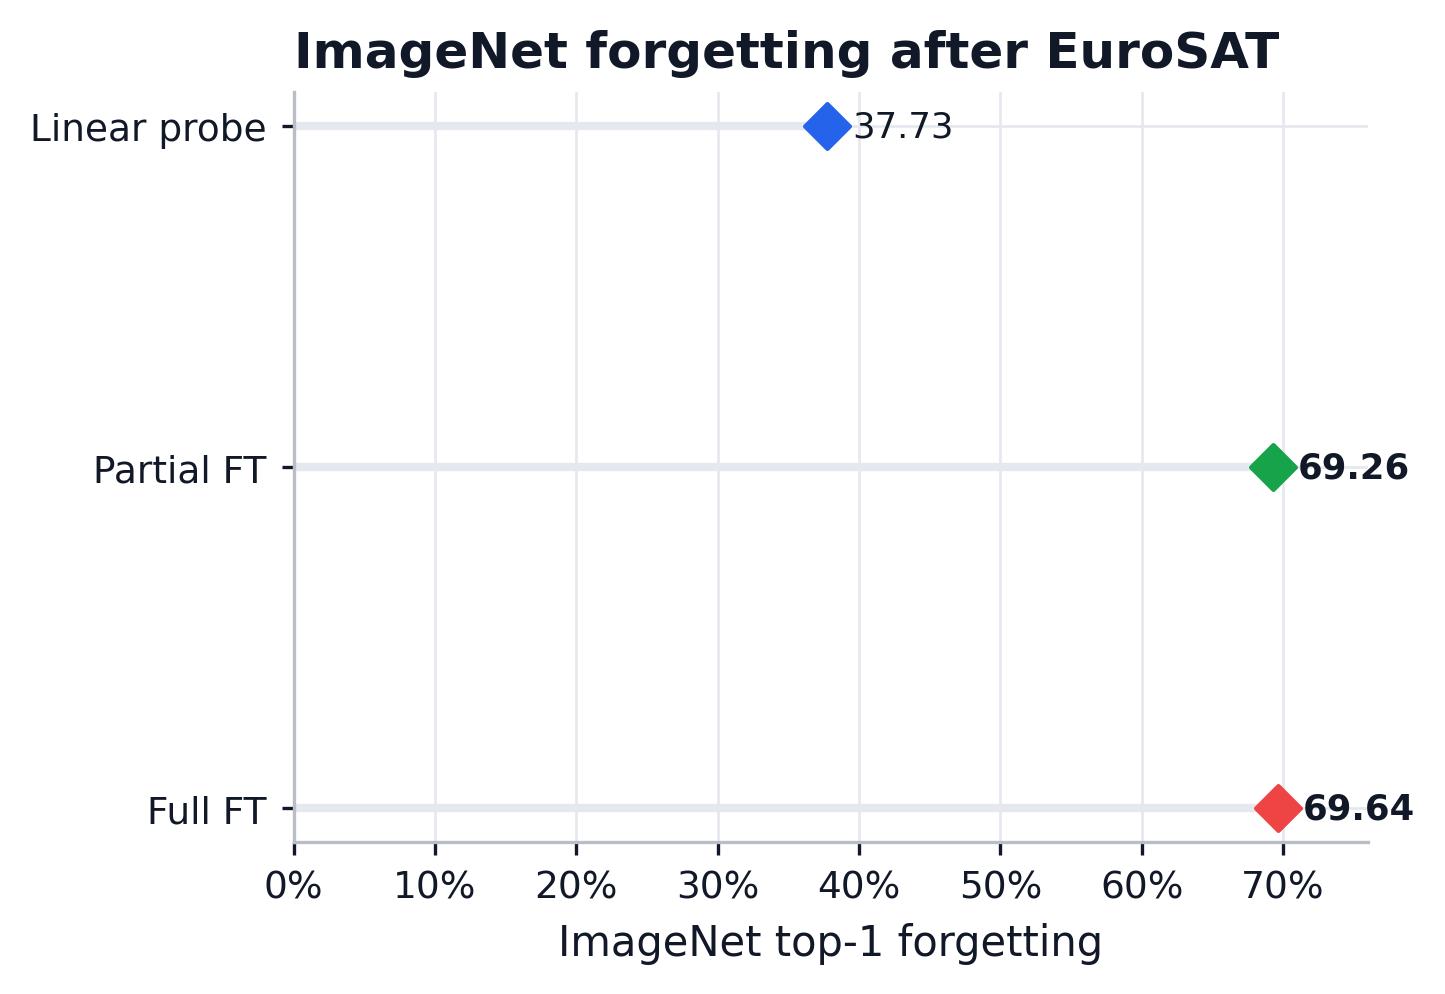
\includegraphics[width=0.92\columnwidth]{../outputs/new_style_picture/forgetting_main/forgetting_top1.png}
\caption{Forgetting after the main EuroSAT experiment. ImageNet top-1 forgetting by transfer strategy.}
\label{fig:forget-main}
\end{figure}

The main forgetting experiment reveals a clear adaptation-retention trade-off. It is worth noting that the magnitude of forgetting is extremely large. After partial unfreezing and full fine-tuning, ImageNet top-1 accuracy falls to below 1\%, suggesting that the adapted backbone becomes almost completely incompatible with the original ImageNet classifier. This result indicates that substantial downstream adaptation can dramatically alter the learned representation, even when downstream performance improves. Future work could investigate the mechanisms behind this extreme forgetting and evaluate mitigation methods designed to preserve source-task knowledge.


\subsection{Forgetting After the Same-Size Cross-Domain Experiment}
This section studies whether forgetting differs between EuroSAT and CIFAR-10 when the downstream sample budget is matched. For each pretrained strategy from Section~4.2, we evaluate the adapted backbone on the official ImageNet validation set and compare it with the original torchvision ResNet-18 baseline. Training from scratch is excluded because it was not initialized from ImageNet.

\begin{table}[!htbp]
\centering
\small
\caption{Forgetting in the same-size cross-domain experiment.}
\label{tab:forgetdomain}
\resizebox{\columnwidth}{!}{%
\begin{tabular}{llrrrrr}
\toprule
Dataset & Strategy & After & Forget & After F1 & Forget F1 & Downstream \\
\midrule
CIFAR-10 & Linear probe & 28.53 & 41.23 & 30.40 & 38.90 & 78.20 \\
CIFAR-10 & Partial unfreeze & 0.59 & 69.17 & 0.35 & 68.95 & \textbf{91.19} \\
CIFAR-10 & Full fine-tune & 0.23 & 69.53 & 0.09 & 69.21 & 90.07 \\
EuroSAT & Linear probe & 32.03 & 37.73 & 33.87 & 35.43 & 88.54 \\
EuroSAT & Partial unfreeze & 0.23 & 69.53 & 0.07 & 69.23 & \textbf{97.51} \\
EuroSAT & Full fine-tune & 0.13 & 69.63 & 0.03 & 69.27 & 97.31 \\
\bottomrule
\end{tabular}}
\vspace{0.15em}
\end{table}

\begin{figure}[!htbp]
\centering
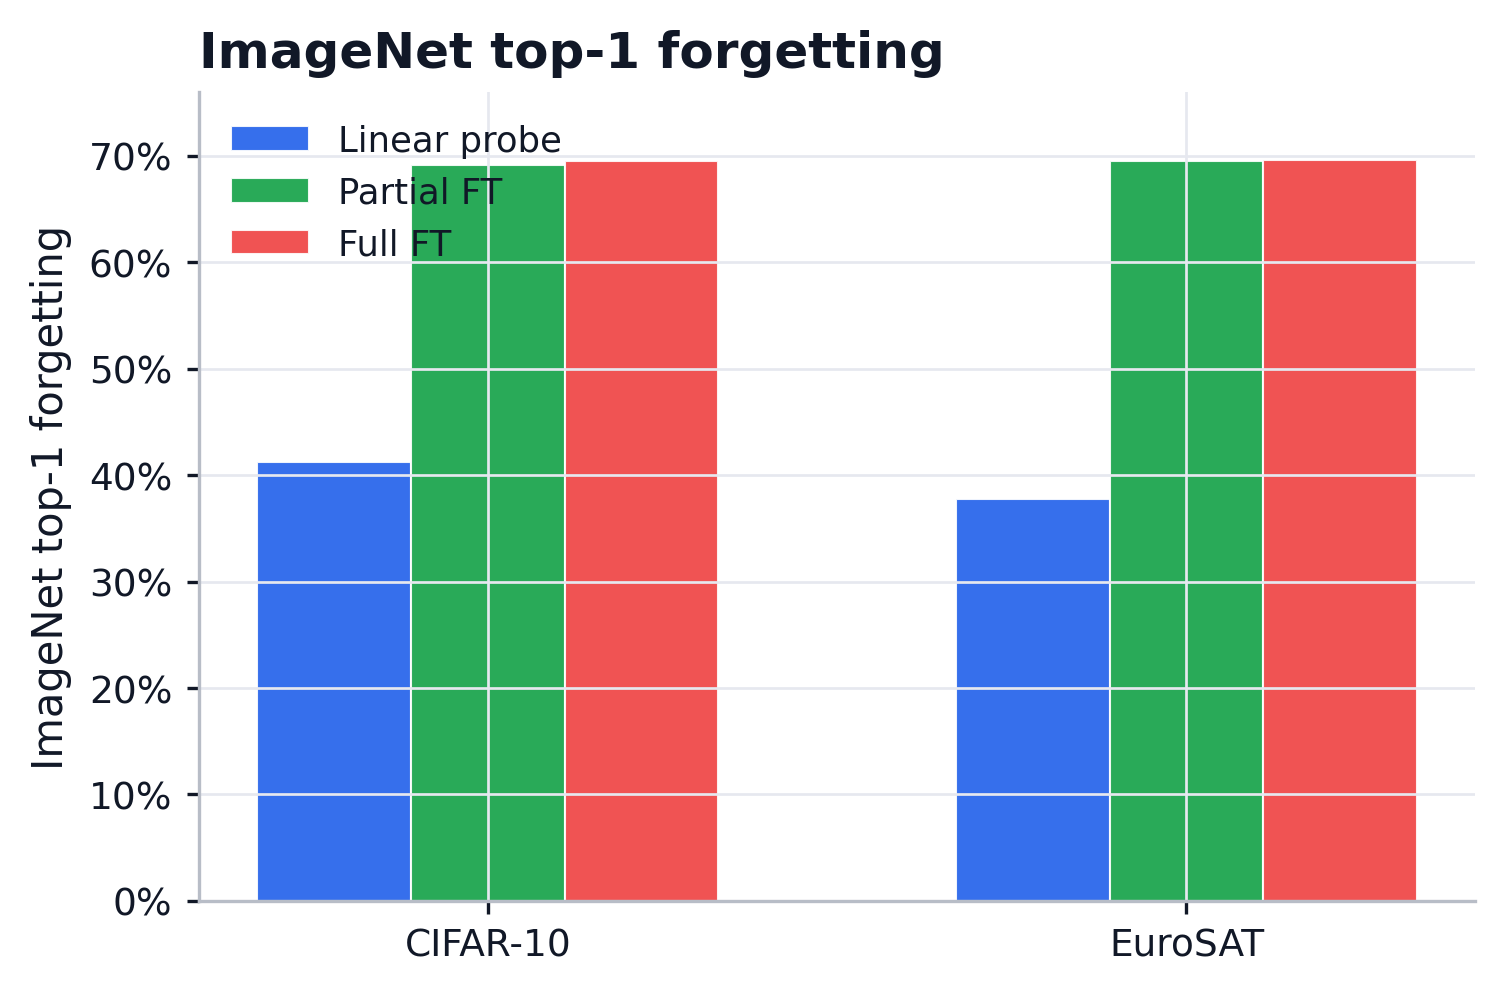
\includegraphics[width=0.82\columnwidth]{../outputs/new_style_picture/forgetting_domain_gap/forgetting_top1.png}
\vspace{0.1em}
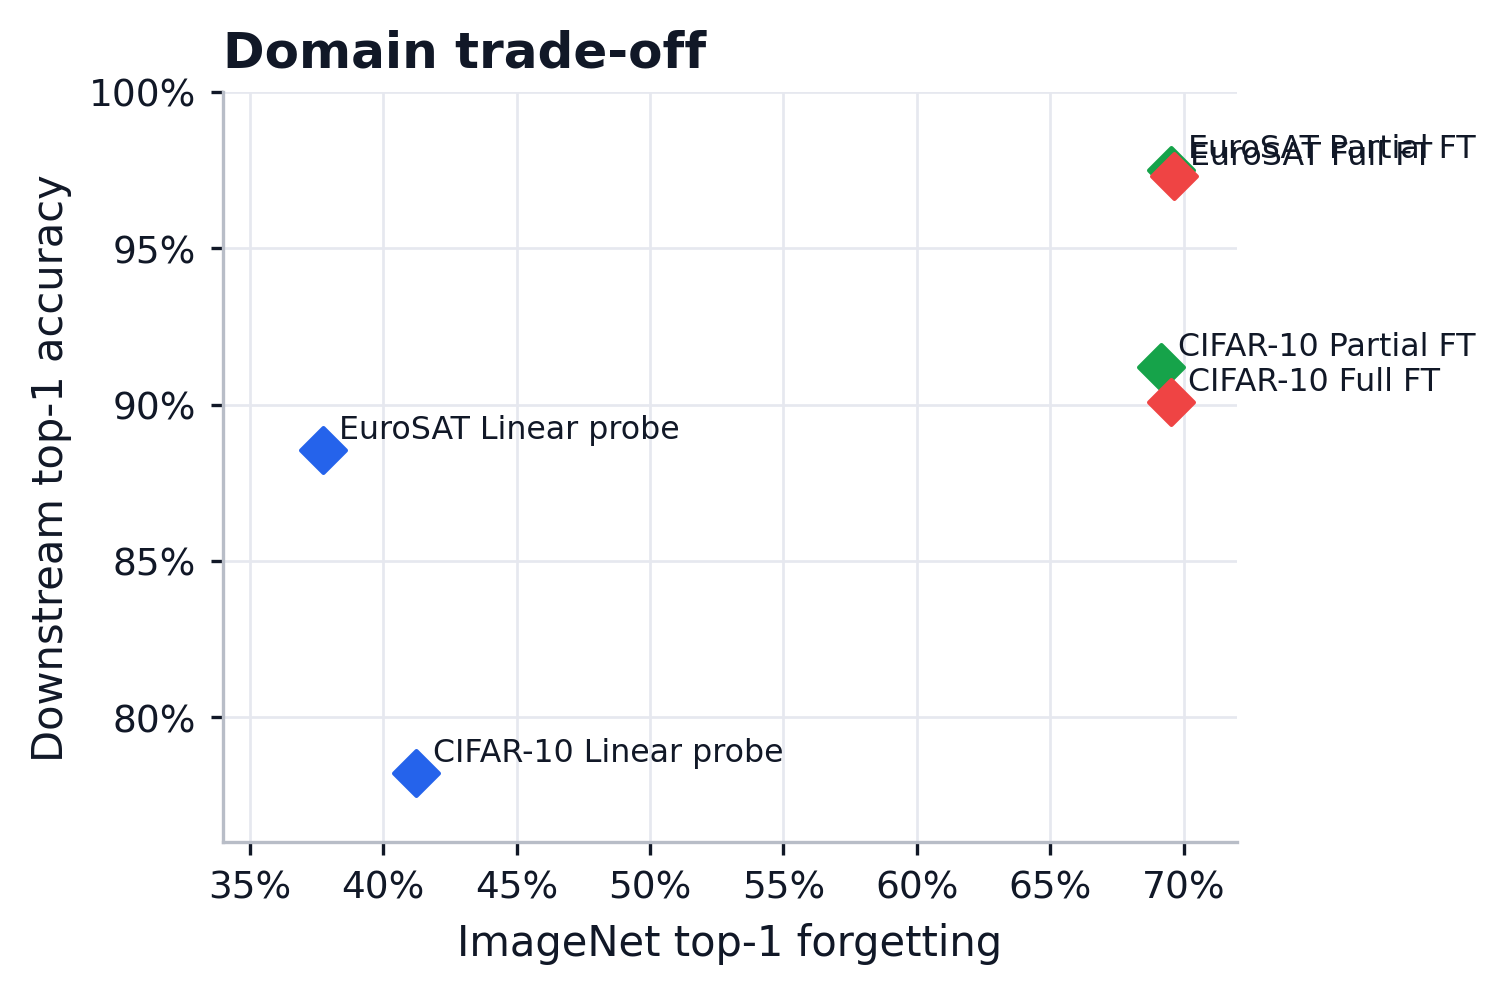
\includegraphics[width=0.82\columnwidth]{../outputs/new_style_picture/forgetting_domain_gap/transfer_forgetting_tradeoff.png}
\caption{Forgetting after same-size downstream adaptation. Top: ImageNet top-1 forgetting. Bottom: downstream accuracy and ImageNet forgetting trade-off.}
\label{fig:forget-domain}
\end{figure}


The forgetting results follow the same strategy-level pattern as Section~5.1. Partial unfreezing and full fine-tuning obtain the strongest downstream accuracy, but both reduce ImageNet top-1 accuracy from 69.76\% to below 1\% on both downstream datasets. Linear probing retains more ImageNet performance because the backbone remains frozen, but it is also the weakest pretrained strategy on the downstream tasks.

The domain-gap forgetting results show that a downstream task being closer to ImageNet does not prevent forgetting after fine-tuning. Although CIFAR-10 is visually closer to ImageNet and receives larger transfer gains, the forgetting results suggest that representation modification during fine-tuning dominates any potential benefit from source-target similarity when the original task is revisited.

\subsection{Forgetting After the Data-Size Experiment}
This section evaluates how forgetting changes as the amount of EuroSAT downstream data increases. Combined with Section~4.3, it allows the report to analyze the trade-off between improved downstream adaptation and greater modification of the pretrained representation. The original ImageNet-pretrained ResNet-18 obtains 69.76\% top-1 accuracy before EuroSAT adaptation, and forgetting is measured as $A_{\text{before}} - A_{\text{after}}$. For consistency with Section~4.3, this section focuses on top-1 forgetting across training fractions.

\begin{table}[!htbp]
\centering
\small
\caption{Forgetting in the EuroSAT data-size experiment.}
\label{tab:forgetfraction}
\begin{tabular}{rlrrr}
\toprule
Train \% & Strategy & After & Forget & EuroSAT \\
\midrule
10 & Linear probe & 32.50 & 37.26 & 76.20 \\
10 & Full fine-tune & 1.24 & 68.52 & 93.58 \\
30 & Linear probe & 32.11 & 37.65 & 85.10 \\
30 & Full fine-tune & 0.25 & 69.51 & 96.65 \\
60 & Linear probe & 31.62 & 38.14 & 86.99 \\
60 & Full fine-tune & 0.25 & 69.51 & 96.88 \\
100 & Linear probe & 32.13 & 37.63 & 87.93 \\
100 & Full fine-tune & 0.20 & 69.56 & 97.15 \\
\bottomrule
\end{tabular}
\end{table}

\begin{figure}[!htbp]
\centering
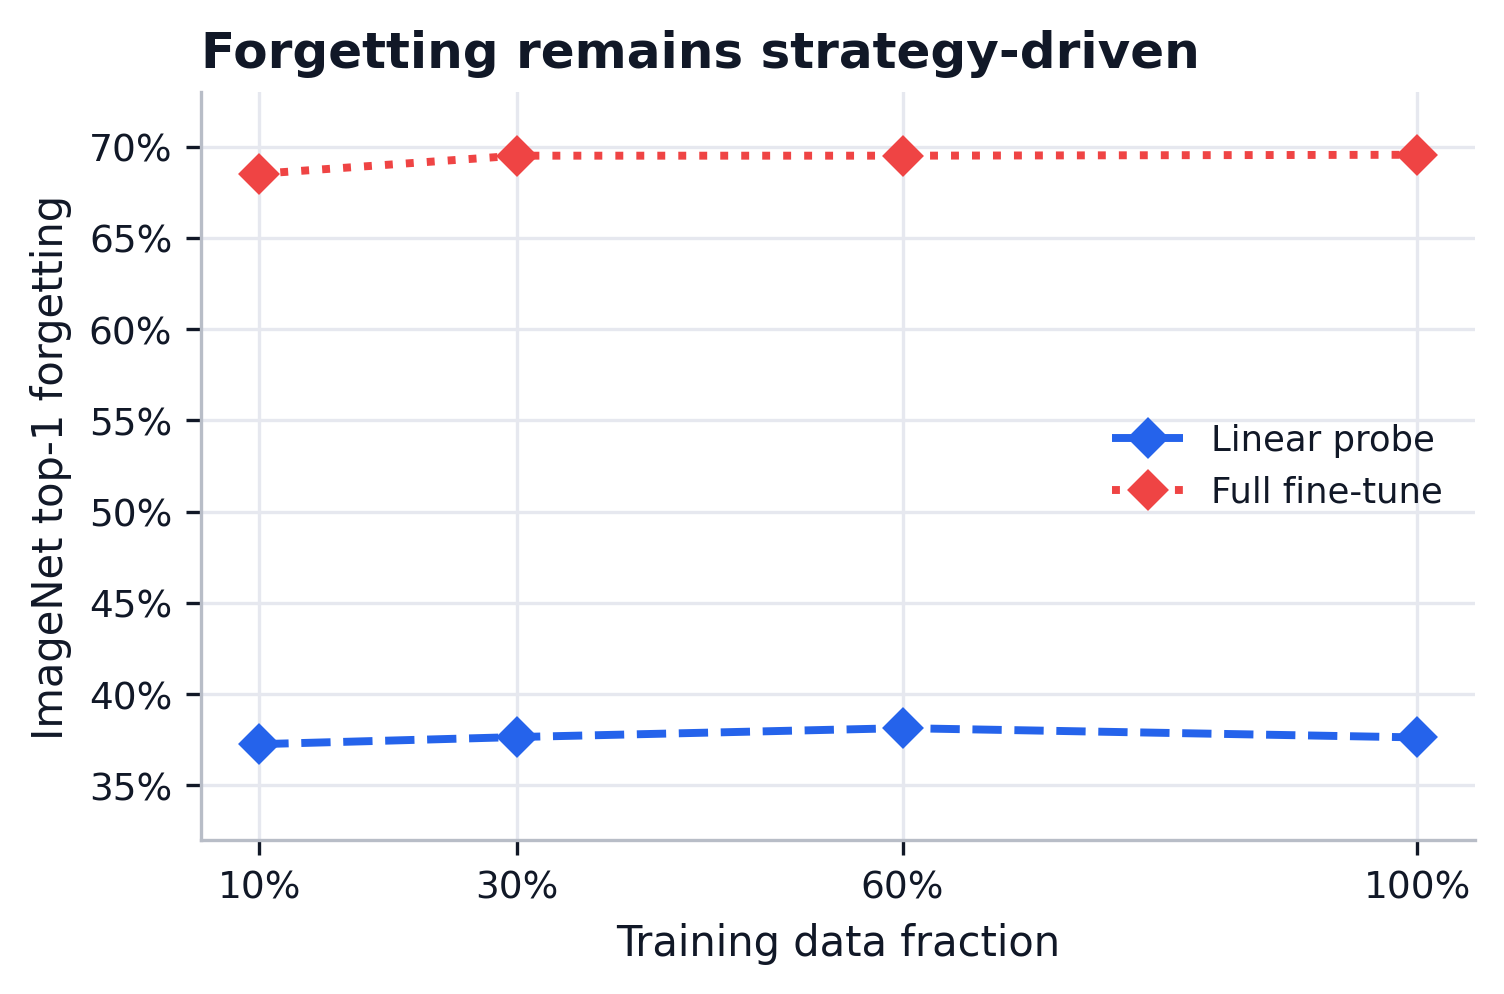
\includegraphics[width=0.82\columnwidth]{../outputs/new_style_picture/forgetting_data_fraction/forgetting_top1_transfer_methods.png}
\vspace{0.1em}
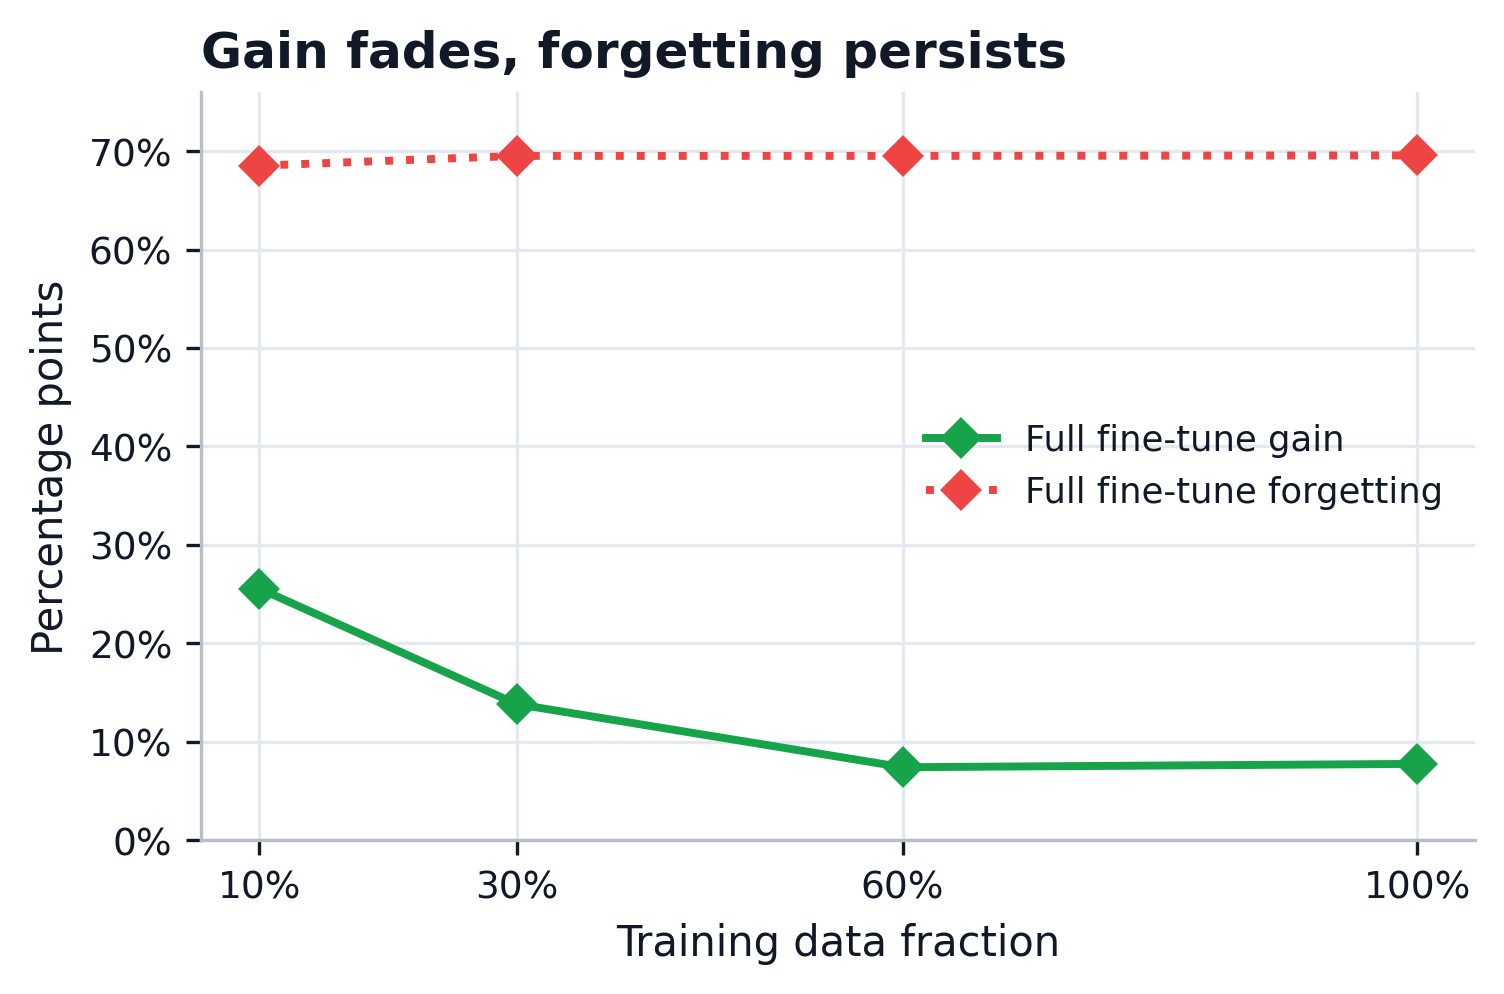
\includegraphics[width=0.82\columnwidth]{../outputs/new_style_picture/forgetting_data_fraction/transfer_forgetting_tradeoff.png}
\caption{Forgetting after the data-size experiment. Top: ImageNet top-1 forgetting by transfer method. Bottom: transfer gain and forgetting trade-off.}
\label{fig:forget-fraction}
\end{figure}


The main result is that forgetting depends more on the training strategy than on the amount of EuroSAT data. Full fine-tuning forgets heavily at every data size: ImageNet top-1 drops from 69.76\% to about 0.20\%--1.24\%, meaning that the adapted backbone is no longer compatible with the original ImageNet classifier.

Linear probing preserves more ImageNet ability. Its ImageNet top-1 stays around 31\%--32\%, giving about 37--38 points of forgetting. The data-size forgetting results show that forgetting is driven more by the fine-tuning strategy than by the amount of EuroSAT data: full fine-tuning forgets heavily at every data fraction, while linear probing preserves more ImageNet accuracy but gives lower EuroSAT performance.


\section{Discussion}
The experimental findings suggest several explanations for when transfer helps and why catastrophic forgetting occurs.

Linear probing performs poorly on EuroSAT because the fixed ImageNet representation is not directly aligned with remote-sensing scene categories. A linear classifier can only draw new boundaries on top of the existing feature space; it cannot reshape features for overhead texture, land-cover patterns, and spatial layout \cite{cheng2020,helber2019}. Linear probing therefore protects the pretrained backbone, but exposes the limitation of frozen features under domain shift.

Partial unfreezing works well because it matches the hierarchy of convolutional networks. Early layers encode reusable primitives such as edges, color contrast, and texture, while deeper residual blocks encode more task-specific combinations \cite{yosinski2014}. Updating only the final residual stage and classifier gives enough flexibility to adapt to EuroSAT without disturbing all low-level filters. Under the short training budget used here, full fine-tuning therefore does not produce a clear EuroSAT advantage over partial unfreezing.

The CIFAR-10 and data-size experiments show that absolute accuracy and transfer gain should be interpreted separately. CIFAR-10 has lower absolute accuracy than EuroSAT, but a larger transfer gain, partly because it shares more natural-image structure with ImageNet while remaining harder after resizing from $32 \times 32$ to $224 \times 224$. In the data-size study, pretrained features act as a useful inductive bias when EuroSAT labels are limited; as the training set grows, the scratch baseline receives more evidence and narrows the gap. Transfer in this project therefore mainly improves sample efficiency.

Catastrophic forgetting arises because fine-tuning optimizes the shared backbone for a new 10-class objective rather than the original 1000-class ImageNet objective. This is consistent with prior observations that training on a new task can reduce performance on a previous task \cite{goodfellow2013}. Linear probing remains on the lower-forgetting side of the trade-off plots because the backbone is frozen, but it also gives weaker downstream accuracy. Partial unfreezing and full fine-tuning move toward higher downstream accuracy while also moving toward the higher-forgetting side, leaving no method in the ideal upper-left region.

The data-size forgetting results add one qualification: increasing EuroSAT data reduces the relative transfer gain, but it does not remove the source-task cost of full fine-tuning. Across all fractions, ImageNet top-1 still falls to about 0.20\%--1.24\%, consistent with evidence that fine-tuning can distort pretrained features under distribution shift \cite{kumar2022}. The non-zero drop under linear probing should also be treated carefully, because frozen convolutional weights may still be paired with shifted BatchNorm running statistics; a frozen-BatchNorm ablation would help separate true representation forgetting from normalization drift \cite{li2016adabn}.

The study has several limitations: it uses a single architecture, a single random seed, and a fixed eight-epoch training budget, and it does not compare mitigation methods such as EWC, Learning without Forgetting, rehearsal, or progressive freezing \cite{kirkpatrick2017,li2016}.

\section{Conclusion}
This project shows that ImageNet transfer can substantially improve EuroSAT classification, but only when the pretrained backbone is allowed to adapt. Partial unfreezing gives the strongest balance of EuroSAT accuracy and efficiency under the training budget used in this project, while linear probing retains more ImageNet ability at the cost of weaker downstream performance.

Transfer is most useful when labelled target data are limited or when the target domain is closer to ImageNet. However, stronger adaptation also causes severe catastrophic forgetting on the original ImageNet task. Future work should therefore focus on mitigation methods that preserve source-task performance while retaining the downstream gains of fine-tuning.

\vspace{0.1em}
\footnotesize
\begin{thebibliography}{10}
\setlength{\itemsep}{0pt}
\setlength{\parskip}{0pt}

\bibitem{yosinski2014}
J.~Yosinski, J.~Clune, Y.~Bengio, and H.~Lipson.
\newblock How transferable are features in deep neural networks?
\newblock In {\em Advances in Neural Information Processing Systems}, pages 3320--3328, 2014.

\bibitem{russakovsky2015}
O.~Russakovsky et~al.
\newblock ImageNet large scale visual recognition challenge.
\newblock {\em International Journal of Computer Vision}, 115(3):211--252, 2015.

\bibitem{deng2009}
J.~Deng et~al.
\newblock ImageNet: A large-scale hierarchical image database.
\newblock In {\em Proceedings of the IEEE Conference on Computer Vision and Pattern Recognition}, pages 248--255, 2009.

\bibitem{cheng2020}
G.~Cheng, X.~Xie, J.~Han, L.~Guo, and G.-S. Xia.
\newblock Remote sensing image scene classification meets deep learning: Challenges, methods, benchmarks, and opportunities.
\newblock {\em IEEE Journal of Selected Topics in Applied Earth Observations and Remote Sensing}, 13:3735--3756, 2020.

\bibitem{helber2019}
P.~Helber, B.~Bischke, A.~Dengel, and D.~Borth.
\newblock EuroSAT: A novel dataset and deep learning benchmark for land use and land cover classification.
\newblock {\em IEEE Journal of Selected Topics in Applied Earth Observations and Remote Sensing}, 12(7):2217--2226, 2019.

\bibitem{he2016}
K.~He, X.~Zhang, S.~Ren, and J.~Sun.
\newblock Deep residual learning for image recognition.
\newblock In {\em Proceedings of the IEEE Conference on Computer Vision and Pattern Recognition}, pages 770--778, 2016.

\bibitem{goodfellow2013}
I.~J. Goodfellow, M.~Mirza, D.~Xiao, A.~Courville, and Y.~Bengio.
\newblock An empirical investigation of catastrophic forgetting in gradient-based neural networks.
\newblock arXiv:1312.6211, 2013.

\bibitem{krizhevsky2009}
A.~Krizhevsky.
\newblock Learning multiple layers of features from tiny images.
\newblock Technical Report, University of Toronto, 2009.

\bibitem{kirkpatrick2017}
J.~Kirkpatrick et~al.
\newblock Overcoming catastrophic forgetting in neural networks.
\newblock {\em Proceedings of the National Academy of Sciences}, 114(13):3521--3526, 2017.

\bibitem{li2016}
Z.~Li and D.~Hoiem.
\newblock Learning without forgetting.
\newblock In {\em European Conference on Computer Vision}, pages 614--629, 2016.

\bibitem{kumar2022}
A.~Kumar, A.~Raghunathan, R.~Jones, T.~Ma, and P.~Liang.
\newblock Fine-tuning can distort pretrained features and underperform out-of-distribution.
\newblock In {\em International Conference on Learning Representations}, 2022.

\bibitem{li2016adabn}
Y.~Li, N.~Wang, J.~Shi, J.~Liu, and X.~Hou.
\newblock Revisiting batch normalization for practical domain adaptation.
\newblock arXiv:1603.04779, 2016.

\end{thebibliography}

\end{document}